\section{Existant Organisationnel}
    \subsection{Structure Organisationnel de GSTP, organigramme}
        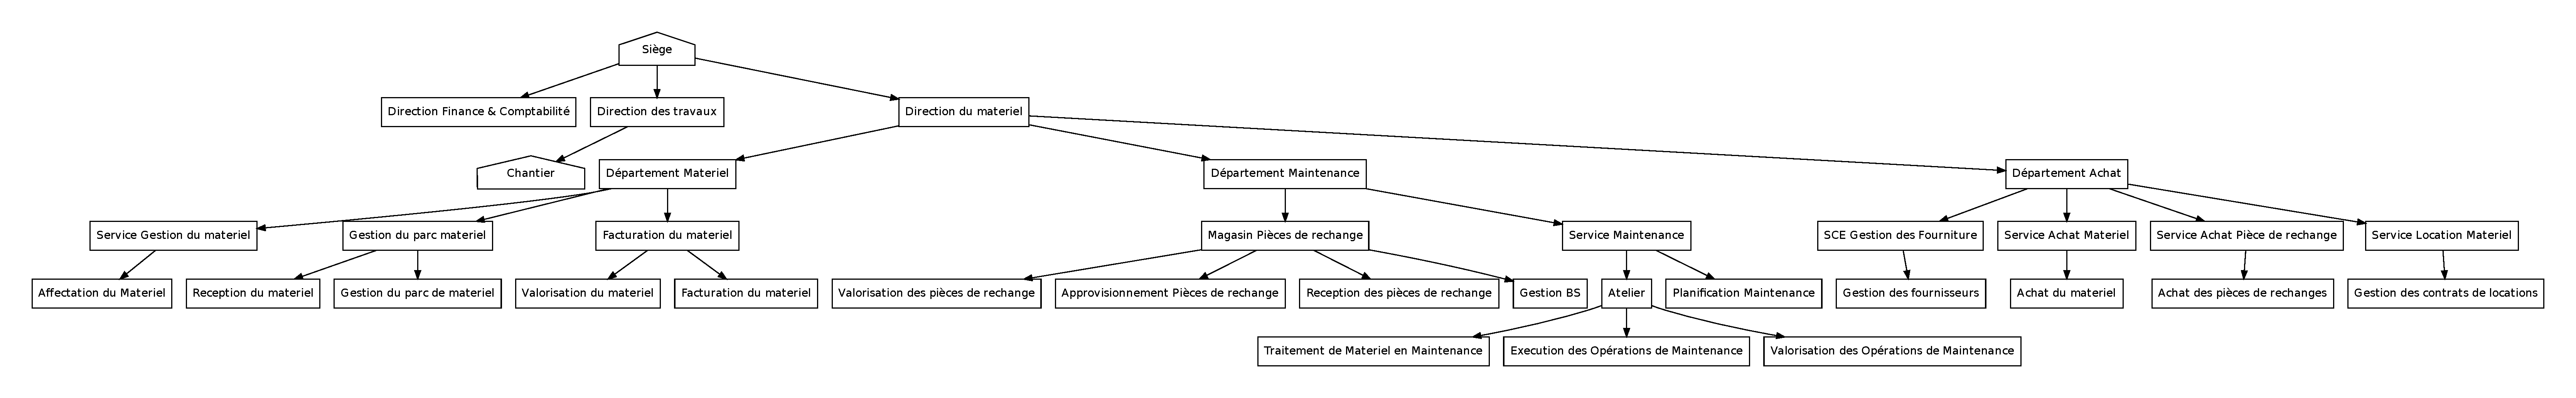
\includegraphics[width=\textwidth]{img/structureOrganisationnel.pdf}

    %%%%%%%%%%%%%%%%%%%%%%%%%%%%%%%%%%%%%%%%%%%%%%%%%%%%%
    %                                                   %
    %   Ce qui suit est recopié directement du sujet.   %
    %   Est-ce fondamentalement grave ?                 %
    %                                                   %
    %%%%%%%%%%%%%%%%%%%%%%%%%%%%%%%%%%%%%%%%%%%%%%%%%%%%%

    \subsection{En détail pour la Direction du Materiel}
        \subsubsection{Rôle global}
            Rattachée à la direction générale, la Direction du Materiel a pour missions de :
            \begin{itemize}
                \item affecter le matériel aux chantiers;
                \item assurer la maintenance et la rénovation du matériel;
                \item gérer le stock de pièces de rechange;
                \item renouveler le matériel (acquisition), avec l'accord de la DG car il s'agit d'un acte d'investissement;
                \item facturer l'utilisation du matériel aux chantiers. La DM joue un rôle de fournisseur (location du matériel) vis-à-vis des chantiers.
            \end{itemize}
            
        \subsubsection{Départements et leur rôles}
            \paragraph{Département Materiel}
                Le département materiel est composé de trois services :
                \subparagraph{Service Gestion du Matériel}
                    Son rôle est de gérer le planning d’affectation et d’assurer l’affectation du matériel aux différents chantiers. Il est consituté de trois personnes.
                \subparagraph{Gestion du Parc Matériel}
                    Il s’occupe de la réception, envoi du matériel et de la gestion du parc matériel. Il est constitué d'une personne.
                \subparagraph{Facturation du Matériel}
                    Ce service s’occupe de la valorisation et de la facturation du matériel. Il est constitué d'une personne.        
                
            \paragraph{Departement Maintenance}
                Il est composé de deux services :
                \subparagraph{Le service gestion des Pièces de Rechange}
                    Son rôle est d’assurer l’approvisionnement, la réception, la valorisation et la gestion des pièces   de rechange. Il y a un magasin au siège de l’entreprise et deux autres délocalisés. Ce service est constitué d'une personne par magasin. 
                \subparagraph{Le service de Maintenance}
                    Il est composé d’une quarantaine d’ateliers et il s’occupe de la planification, de l’exécution et de la valorisation des opérations de maintenance et des divers traitements. Ce service est constitué de 60 personnes répartis sur 40 ateliers (dont 8 à l’atelier principal, et les autres étant repartis sur les ateliers de chantiers).
Le processus de maintenance est composé de :
\begin{itemize}
	\item Effectuer les opérations de maintenance urgentes (depuis de demandes des chantiers)
\item Procéder au remplacement d'un matériel en panne 
\item Réaliser la planification de maintenance préventive
\end{itemize}
	Il se déroule comme suivant :

Lors d’une demande de maintenance planifiée ou  depuis un chantier, on procède en identifiant les opérations à effectuer. Ou lors d’une demande d’intervention urgente depuis un chantier, on diagnostique la panne, dans le cas de nécessité, on réalise une demande de matériel urgente.
Suivant la disponibilité du personnel, on affecte l’opération. Si l’opération nécessite des pièces de rechange, on signale pour les obtenir.
A la fin de l’opération on signale au chantier ou au parc matériel que l’objet de la maintenance est à nouveau disponible (et en état de marche…).
Au niveau d’informatique : 
\begin{itemize}
	\item Logicielle : Il est équipé une application de gestion de stocks de pièce de rechange (+6000 références) une autre application de planification de la maintenance.
\item Matérielle : Il est doté 2 imprimantes et 2 PCs connectés au réseau de la Direction Matérielle.
\end{itemize}

            \paragraph{Departement Achat}
                Le département achat est constitué de quatres services :

                \subparagraph{Service Gestion des Fournisseurs}
	                C'est le service qui va être en communication avec les fournisseurs de matériel afin d'avoir les meilleurs matériels sur le marché aux moindres coûts.
                \subparagraph{Service d’Achat du Matériel}
	                Ce service s'occupe des achats de nouveaux matériels.
                \subparagraph{Service d’Achat des pièces de Rechange}
	                Ce service s'occupe de tous les achats de pièces de rechange.
                \subparagraph{Service Location du Matériel}
	                Ce service s'occupe des locations de matériels lorsque le parc n'offre pas suffisamment de disponibilités pour répondre à un besoin d'un chantier. Il peut également s’occuper de l’achat d’autres prestations (maintenance, etc.)
